ในการสร้างโมเดลปัญญาประดิษฐ์นั้นการใช้จำนวนชั้น (layer) เยอะนั้นจะทำให้ได้คุณลักษณะของข้อมูลที่ออกมาเยอะตามไปด้วย แต่การที่คุณลักษณะของข้อมูลเยอะไม่ได้หมายความว่าโมเดลปัญญาประดิษฐ์จะให้ประสิทธิภาพที่ดีเสมอไป ซึ่งสามารถแก้ปัญหานี้ได้โดยใช้ Residual Network (ResNet) ที่เป็น Convolution Neuron Network (CNN) ประเภทหนึ่ง ที่ส่วนใหญ่จะนำมาใช้กับข้อมูลที่เป็นรูปภาพ เช่น การจดจำวัตถุ เป็นต้น โดย ResNet นี้จะสามารถทำการข้ามชั้นของ CNN ที่ไม่จำเป็นได้ โดยในชั้นที่ไม่จำเป็นจะมีการปรับ weight ให้เข้าใกล้ 0 ในขณะที่ train ข้อมูล การข้ามชั้น CNN ที่ไม่จำเป็นจะช่วยลดเวลาที่ใช้ในการ train และทำให้ประสิทธิภาพของโมเดลปัญญาประดิษฐ์ดีขึ้น

\begin{figure}[!ht]
	\centering
	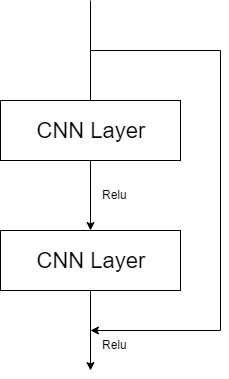
\includegraphics[width=0.2\textwidth]{chapter2/images/example_resnet.png}
		\caption{ResNet}
    	\label{fig:ResNet}
\end{figure}

การทดลองโมเดลปัญญาประดิษฐ์ ResNet ด้วยการทำจำแนกรูปภาพโดยใช้ชุดข้อมูลของ ImageNet ที่ประกอบไป class มากว่า 1,000 class มาเทียบกับโมเดลปัญญาประดิษฐ์ทั่วไป (plain) ที่จำนวนชั้น 18 ชั้น และ 34 ชั้น ผลลัพท์จะได้ออกมาตามตารางด้านล่างดังนี้ (โครงสร้างพื้นฐานของโมเดลปัญญาดิษฐ์ ResNet และโมเดลปัญญาประดิษฐ์ทั่วไปเหมือนกัน)

\begin{table}[!ht]
	\centering
	\begin{tabular}{|c|c|c|}
		\hline
		{จำนวนชั้นของ}&\multicolumn{2}{c|}{training error}\\
		\cline{2-3}
		{}							& plain						& ResNet				\\
		\hline
		18							& 27.94						& 27.88				\\
		34							& 28.54						& 25.03				\\
		\hline
	\end{tabular}
	\caption{Top-1 ของความผิดพลาดของชุดข้อมูลทดสอบ ImageNet}
	\label{tab: Top-1 error of ImageNet}
\end{table}

จากตาราง \ref{tab: Top-1 error of ImageNet} จะเห็นได้ว่าโมเดลปัญญาประดิษฐ์ทั่วไป 34 ชั้นมีค่าเปอเซนต์ความผิดพลาดสูงกว่าโมเดลปัญญาประดิษฐ์ ResNet แบบชัดเจน ในขณะที่โมเดลปัญญาประดิษฐ์ทั่วไปจะมีเปอเซนต์ความผิดพลาดสูงขึ้นเมื่อเทียบกันระหว่าง 18 ชั้นและ 34 ชั้น
\par
ต่อมาจะนำโมเดลปัญญาประดิษฐ์ ResNet มาทดสอบกับชุดข้อมูล CIFAR-10 ซึ่งเป็นชุดข้อมูลที่มีภาพสำหรับ train 50,000 ภาพ ภาพสำหรับทดสอบ 10,000 ภาพ และมีจำนวน class ทั้งหมด 10 class โดยจะมีการออกแบบของจำนวนชั้นของโมเดลปัญญาประดิษฐ์ ResNet ตามจำนวนของชั้น Convolution ที่มีผังคุณลักษณะเท่ากัน 6 ชั้นติดกันและการข้ามชั้นที่ละ 2 จึงทำให้ได้รูปแบบการคิดชั้นดังนี้ 6n + 2 สำหรับการทดสอบจะให้ค่า n = [3,5,7,9,200] ดังตารางต่อไปนี้

\begin{table}[!ht]
	\centering
	\begin{tabular}{|c|c|c|}
		\hline
		{โมเดลปัญญาประดิษฐ์}				&{จำนวนชั้น}					&{training error}		\\
		\hline
		ResNet						& 20							& 8.75				\\
		ResNet						& 32							& 7.51				\\
		ResNet						& 44							& 7.17				\\
		ResNet						& 56							& 6.97				\\
		ResNet						& 110						& 6.43				\\
		ResNet						& 1202						& 7.93				\\
		\hline
	\end{tabular}
	\caption{ค่าความผิดพลาดที่ได้จากการทดลองจำนวนชั้นของโมเดลปัญญาประดิษฐ์ ResNet บนชุดของข้อมูล CIFAR-10}
	\label{tab: Classification error}
\end{table}
จากตาราง \ref{tab: Classification error} จะเห็นได้ว่าที่ีโมเดลปัญญาประดิษฐ์ ResNet ที่มีจำนวนชั้น 1202 นั้นมีค่าความผิดพลาดเกิดขึ้นมากกว่าจำนวนชั้น 110 ซึ่งอาจจะเป็นไปได้ว่าขนาดของโมเดลปัญญาประดิษฐ์ ResNet ที่มีจำนวนชั้น 1202 นั้นมากเกินไปสำหรับชุดข้อมูลขนาดเล็กนี้